\chapter{Background}\label{chap:bkgnd}

\section{Jingju music}
Jingju (also known as Beijing or Peking opera) is the most representative form of Chinese opera which assimilates the essence of various Chinese opera forms such as 徽剧 (Anhui opera), 昆曲 (Kun opera), 秦腔 (Qin qiang) and 高腔 (Gao qiang). It arose in the late 18th century and became fully developed in the mid-19th century. Now it is regarded one of the cultural treasures in China and inscribed in the UNESCO representative list of the intangible cultural heritage of humanity. Jingju is widely practised over mainland China, Hong Kong, Taiwan, and overseas countries where there is Chinese communities presence. Major jingju performing troupes are located in big mainland China cities such as Beijing, Tianjin and Shanghai. A significant amount of jingju musicological literature can be used to formulate MIR problems. The presence of a large audience and musicological literature are an important motivation to carry a computational research for this music culture.

This section describes the focus of this dissertation -- jingju music culture. The emphasis is on singing concepts in this music culture. This section is not a comprehensive introduction to this culture but is aimed to be sufficient to support the following chapters of the dissertation.

We use simplified Chinese characters (computer encoding: GB2312) to introduce jingju terminologies for the first time in this dissertation. We also introduce the pinyin, the romanization system of Mandarin Chinese, for each terminology. Only the pinyin form of the terminology will be used throughout the dissertation. 

\subsection{A synthetic art form}

Professor Li in National Academy of Chinese Theatre Arts (NACTA) said ``The three basic elements of Chinese opera are 曲 (pinyin: qu, tune), 程式 (pinyin: chengshi, conventions -- a strict set of rules) and 虚拟表演 (pinyin: xu ni biao yan, virtual acting). These three elements are ultimately aiming to support 戏 (pinyin: xi), which can be approximately understood as `entertainment'." Of the three elements, ``tune" is the most important one, which represents all the musical dimensions of the jingju music. However, this representation is not only limited to music but constructs the whole skeleton of the jingju performing.

Jingju is a synthetic art form which includes four disciplines -- 唱 (pinyin: chang, singing),念 (pinyin: nian, declamation),做 (pinyin: zuo, physical acting) and 打 (pinyin: da, acrobatics). Singing is directly related to tune, and the other three disciplines are integrated together by the music and rhythm of jingju performing. 

The jingju technical training for performers consists in becoming proficient of the conventions of the four disciplines as mentioned earlier which are established by tradition. The jingju performers use these conventions to construct characters and convey stories. For example, they use singing conventions to express the character's emotional state. The jingju performance is codified through the conventions which are not aimed at hinder the creativity and artistry. The appreciation of the beauty of jingju is to see how the performers are conveying the conventions. In jingju training, a performer will have more creativity if she/he can master more conventions.

\subsection{Singing and instrumental accompaniment}

``In the aural performance of Beijing opera, two types of sounds are actually heard: song and speech vocalized by the stage performers, and instrumental music played by the musicians of the orchestra. The voice of the Beijing opera performer, is the featured component of aural performance." -- Elizabeth Wichmann \cite{Wichmann1991a}.

In a jingju play, the sections where singing occurs are 唱段 (pinyin: chang duan, literally translated as singing section). The closest form to chang duan in Western opera is "aria", which signifies "any closed lyrical piece for solo voice (exceptionally for more than one voice) with or without instrumental accompaniment, either independent or forming part of an opera, oratorio, cantata or other large work." The difference between chang duan and aria is that latter is a self-sufficient piece conceptually, whereas chang duan is formulated in a dramatic continuum, although it is usually performed and recorded individually \cite{Repetto2018}. 

Jingju chang duan is started actually before the performer starts to sing. The declaration of the starting point of a chang duan is 叫板 (pinyin: jiaoban, literally translated as "calling the banshi"). Banshi is the rhythmic framework concept that we will introduce it in \secref{sec:banshi}. Jiaoban is included in every chang duan of the commercial recordings and teached in conservatory jingju performing classes. The percussion pattern 住头 (pinyin: zhu tou) is to signal the end of a chang duan \cite{Mu2007a}.

Jingju instrumental ensemble is divided into two sections -- 文场 (pinyin: wenchang, literally translated as "civil scene") and 武场 (pinyin: wuchang, literally translated as "martial scene"). Wenchang is the orchestral accompaniment, and wuchang is formed by percussion instruments. There are five basic percussion instruments -- 单皮鼓 (pinyin: danpigu, drum), 板 (pinyin: ban, clappers), 铙钹 (pinyin: naobo, cymbals), 大锣 (pinyin: daluo, big gong), 小锣 (pinyin: xiaoluo, small gong). The first two instruments are played normal by the same person, so they have a combined term -- bangu. The musician who plays the bangu is called 司鼓 (pinyin: si gu), literally translated as "the man who is in charge of the bangu". The primary functions of wuchang are playing 锣鼓经 (pinyin: luo gu jing, rhythm patterns) and supporting the rhythmic aspect of the actor/actress’ performing.

The main instrument of wenchang is 京胡 (pinyin: jinghu). Having loud volume, and very bright and penetrating sound, jinghu is the aural representative of jingju sound. The musician who plays jinghu is called 琴师 (pinyin: qin shi, master instrumentalist). The major role played by qinshi is supporting the jingju melody. Traditionally, qinshi is the musician who has the closest collaboration with the performer. Jingju line sustains the singing line to form an uninterrupted melody stream, which impels the singing \cite{Repetto2018}. 

The other instruments in wenchang are 月琴 (pinyin: yueqin), 三弦 (pinyin: sanxian), 京二胡 (pinyin: jingerhu), 阮 (pinyin: ruan), 中阮 (pinyin: zhongruan) and 大阮 (pinyin: daruan). They all play the same melody as the jinghu line in the same or different octave, and in a heterophonic structure. The performer, sigu and qinshi take turns in coordinating the jingju performing tempo.

\subsection{Lyrics structure}\label{sec:ch2:lyrics_structure}

The primary function of the lyrics in jingju is telling stories. Music structure in jingju is closely related to lyrics structure. The tune sequences in jingju are inherited from the creation principle in poetry of Tang dynasty (618 - 907 AC), that the melody and poetic structure are taken from the preexisting poems or songs, and new lyrics are arranged to fit in that schema \cite{Repetto2018}. The new lyrics are labelled with the name of the original poem or song, so that the performer knows how to sing the tune. The label of the original poem or song is called 曲牌 (pinyin: qu pai, literally translated as tune label). Different qupai have different forms which represent not only different melodies but also a different number of melodic lines and a different number of characters in each line. This kind of lyrics structure is called 长短句 (pinyin: chang duan ju, literally translated as long and short lines). A jingju chang duan consists of a sequence of these chang duan ju.

The basic structure of lyrics stanza consists of two symmetrical lines which have the same number of characters. The most common term in jingju circles for describing this two symmetrical lines is 上下句 (pinyin: shang xia ju, literally translated as upper and lower lines). The most common English terminology for shang xia ju is couplet for the stanze, opening line for upper line and closing line for lower line \cite{Repetto2018}. A standard line has either 7 or 10 characters, grouped in three sections -- 2 + 2 + 3 or 3 + 3 + 4. These sections, namely 逗 (pinyin: dou), are the basic semantic and rhythmic units \cite{Wichmann1991a}.

The lyrics structure mentioned above can be modified in actual singing. A typical case is the variation of the number of characters in each line, for example, 衬字 (pinyin: chenzi), the characters do not have semantic meaning, but serve to help the performer prolong the singing of certain nasal or vowel sounds. Another form of increasing the number of characters is 垛字 (pinyin: duozi), which inserts semantic units containing 3 or 4 characters into the line.

\subsection{Linguistic tones and pronunciation}\label{sec:linguistic_tones}

It is commonly assumed that the linguistic intonation of a tonal language singing needs to agree with its melody to a certain extent to make sure the intelligibility. For jingju which is sung by using mainly Chinese Mandarin language and various dialects, its music features are related to the dialects. In other words, The Chinese dialects used in jingju singing determines its melody characteristics to a certain extent.

In jingju circles, it exists an expression to describe the relation between linguistic tones and melody -- 字正腔圆 (pinyin: zi zheng qiang yuan, literally translated as “characters should be straight, tune should be round.”). This expression can be understood as that the performer needs to attain both the intelligibility of the lyrics and the smooth sounding of the melody. The most critical problem to be avoided in jingju singing is 倒字 (pinyin: dao zi, literally translated as upside-down character), which means that the lyrics is misunderstood because the performer mispronounces certain characters.

Most of the jingju scholars agree in that jingju singing uses mainly two Chinese dialects -- 北京音 (pinyin: Beijing yin, the dialect of Beijing) and 湖广音 (pinyin: Huguang yin, the dialect of Huguang). Some scholars consider that jingju singing also uses a third Chinese dialect -- 中州韵 (pinyin: Zhongzhou yun, literally translated as rhymes from Zhongzhou). All three dialects share the same tone categories 阴平 (yin ping), 阳平 (yang ping), 上 (shang) and 去 (qu), although the pitch contours of the same characters realized in the same categories are different for the three dialects.

The three dialects result in the complexity of the pronunciation in jingju singing. Such complexity influences the linguistic tones as well as the pronunciation of the syllabic initials and finals. The standard Chinese used in Mainland China -- 普通话 (pinyin: pu tong hua), very close to Beijing yin, is taken as the reference for jingju pronunciation. All the special pronunciations different from the reference putonghua can be divided into two categories -- 尖团字 (pinyin: jian tuan zi, literally translated as pointed and rounded characters) and 上口字 (pinyin: shang kou zi, literally "up to the mouth" characters). Jian tuan zi has two sub-categories of characters -- 尖字 (pinyin: jianzi) and 团字 (pinyin: tuanzi), which are separated by the fricative and affricative consonants of a syllable. When studying a new play, jingju performer should learn which characters belonging to tuanzi in putonghua should be pronounced as jianzi. The jian tuan zi qualities are considered extremely important for both listening comprehension and aesthetic effect \cite{Repetto2018}. Shang kou zi are generally a set of characters of which the pronunciation is different from the standard Mandarin, adopting from southern Chinese dialects -- Huguang yin and Zhongzhou yun. By shang kou zi and converting certain tuanzi to jianzi, the language of jingju is made more appealing to speakers of the diverse range of dialects throughout China than is Mandarin alone \cite{Wichmann1991a}. Jian tuan zi and shang kou zi are one of the main study focuses of this dissertation. Thus a more specific extended description will be presented in section. 

\subsection{Role-types}

行当 (pinyin: hang dang), commonly translated as role-type, is a colloquial term for the “acting profiles” of a jingju performing character. There are four role-types in jingju -- 生 (sheng), 旦 (dan), 净 (jing) and 丑 (chou), which respectively have their specific styles of performing, speaking, singing, costume, and make-up. These oral and visual means of expression define the gender, approximate age, social status, profession, personality and singing style \cite{Yung1989a}. Due to the various and complicate conventions that each role-type possesses, every performer has to specialize one role-type and practice these conventions along the performing career. 

\begin{table}[ht!]
\centering
\begin{tabular}{l|cccc}
\toprule
Main role-types & sheng               & dan                           & jing & chou \\
\midrule
\multirow{4}{*}{Sub role-types} & laosheng\textsuperscript{*} & qingyi\textsuperscript{*} & tongchui    & wenchou   \\
& xiaosheng & huadan & jiazi & wuchou \\
&&laodan&& \\
&&wudan&& \\
\bottomrule
\end{tabular}
\caption{Jingju four role-types and their sub role-types. The role-types with * superscript are the main research objects of this dissertation because singing is their major discipline.}
\label{tab:role-types}
\end{table}

Sheng role-type is specialized in the performance of male characters, whereas dan role-type is specialized in that of female characters. Jing role-type depicts the male characters with an exaggerated temperament. Chou role-type is used for male or female comic characters \cite{Repetto2018}. The most obvious difference between the male’s voice and the female’s voice is the timbre. Male role-types sing with chest voice, while female role-types use falsetto. Regarding the singing pitch register, there is a displacement of the pitch range in the female singing to a higher region, where female sings a fourth to an octave higher than male singing. Regarding melodic contours, female singing is usually more melismatic than male singing \cite{Wichmann1991a}. 

老生 (pinyin: lao sheng) role-type portrays adult or old male characters, which is also the representative of male singing. All textbooks use the examples of laosheng role-type to explain elements of jingju music system. Two representative sub-role-types in dan are 青衣 (pinyin: qing yi) and 花旦 (pinyin: hua dan). The former is most representative role-type of female singing, and generally used for building female characters from a higher social classes. The latter is used for building female characters with a playful personality.

We list the major jingju role-types in \tabref{tab:role-types}, where laosheng and qingyi are the main research objects of this dissertation since singing is their major discipline.

\subsection{Shengqiang}

There is no a coherent definition of jingju 声腔 (pinyin: shengqiang) between scholars. Some of them define shengqiang as tune families of jingju music, meaning a tune which has been evolved into different versions in the performing and transmission process throughout the history. Although these tunes share certain tonal, modal, and dramatic function, they tend to differ from each other in metrical, rhythmic, and melodic details \cite{Yung1989a}. The shengqiang definition of Elizabeth Wichmann deviated from tune family, and characterize a group of related shengqiang as system. Each shengqiang system is identified by its unique patterns of modal rhythm, song structure, melodic contour and construction, and keys and cadences \cite{Wichmann1991a}.  

Jingju contains mainly eight shengqiang -- 西皮 (xipi), 二黄 (erhuang), 反西皮 (fanxipi), 反二黄 (fanerhuang), 四平调 (sipingdiao), 南梆子 (nanbangzi), 高拨子 (gaobozi) and 吹腔 (chuiqiang). Two shengqiang with the most significant presence in jingju arias are xipi and erhuang. Fanxipi and fanerhuang are respectively first degree shifted versions of xipi and erhuang. Additionally, shengqiang is related to the emotional content of the aria. For example, Wichmann describes the emotional content of erhuang as dark, deep, profound, heavy and meticulous, and xipi as sprightly, bright, clear, energetic, forceful, purposeful \cite{Wichmann1991a}. 

\subsection{Banshi}\label{sec:banshi}

Ban means the percussion instrument clappers used in jingju wuchang. Banshi can be understood as the jingju rhythmic patterns.  There are four types of banshi in jingju -- 一板一眼 (one ban and one eye), 一板三眼 (one ban and three eyes), 有板无眼 (ban but no eye) and 无板无眼 (no ban and no yan), where ban and eye indicate respectively accented and unaccented beats. The first three banshi are metred types, and usually notated in jianpu scores correspondingly with the time signatures 2/4, 4/4 and 1/4. The last is assigned to 散板 (pinyin: sanban), meaning unmetred type. Wichmann describes that each banshi has a characteristic tempo, is associated with certain characteristic melodic tendencies, and is perceived as appropriate for certain dramatic situations \cite{Wichmann1991a}. 

\begin{table}[ht!]
\centering
\begin{tabular}{cccc}
\toprule
Tempo & Banshi               & Time signature                           & Melodic tendencies  \\
\midrule
slow & manban & 4/4 & melismatic\\
\multirow{5}{*}{
\includegraphics[width=0.06\textwidth]{figs/shapes/vertical_double_arrow.png}}& zhongsanyan & 4/4 & \multirow{5}{*}{
\includegraphics[width=0.06\textwidth]{figs/shapes/vertical_double_arrow.png}} \\
& kuaisanyan & 4/4 & \\
& yuanban & 2/4 & \\
& erliu & 2/4 & \\
& liushui & 1/4 & \\
fast & kuaiban & 1/4 & syllabic \\
\bottomrule
\end{tabular}
\caption{Jingju metred banshi.}
\label{tab:banshi}
\end{table}

The primary or original banshi is called 原板 (pinyin: yuanban), with time signature 4/4. When it is transformed into 1/4, the corresponding banshi is 快板 (pinyin), and the tempo is also accelerated. When yuanban is transformed into 4/4, the resulting banshi is 慢板 (pinyin: manban), meaning slow banshi. When yuanban is transformed into manban, not only the time duration of syllables are extended, but also the number of ornamentations within each syllable are increased. However, when yuanban is converted to kuaiban, the singing style becomes almost syllabic -- one beat for one syllable. 

三眼 (pinyin: sanyan, literally translated as three eyes) is another name for manban. Sanyan banshi can be divided into three sub-banshi -- 慢三眼 (mansanyan, equal to manban), 中三眼 (zhongsanyan), 快三眼 (kuaisanyan). The tempo of kuaisanyan is faster than zhongsanyan, and they both faster than mansanyan but slower than yuanban. Except for yuanban, the banshi of time signature 2/4 category also contain 二六 (pinyin: erliu, literally translated as two six) because their couplet has six accented beats. In terms of shengqiang xipi, there is another metred banshi -- 流水 (pinyin: liushui, literally running water) which uses 1/4 time signature, is faster than yuanban but slower than kuaiban. We list major jingju metred banshi in \tabref{tab:banshi}.

Three main unmetred banshi are 导板 (daoban), 回龙 (huilong) and 哭头 (kutou). Daoban is the first melodic line of a chang duan. Huilong follows daoban, and is used to draw out the metred banshi. Kutou, literally crying head, is used for a grievous outburst and can occur after any section of the couplet \cite{Repetto2018}. The variety of banshi is needed to convey the emotional content of the lyrics. In general, yuanban is related to neutral and narrative lyrics content; manban reflects introspective, and deep emotions; while kuaiban expresses agitation, nervousness.

The precise, clear pronunciation is critical to jingju listening comprehension, and also form an important aural aesthetic value of jingju. The primary focus of this dissertation is the pronunciation aspect of jingju singing. An in-depth description of jingju pronunciation concepts is given in the following section.

\section{Pronunciation in jingju singing}

Mandarin is a tonal language and there are in general 4 lexical tones and 1 neutral tone in it. Every character of spoken Mandarin language is pronounced as mono-syllable \cite{lin_new_1993}. When the differences in tones are disregarded, the total number of different pronounced syllables is 408. The jingju singing is the most precisely articulated rendition of the spoken Mandarin language. Basic pronunciation of a jingju syllable is categorized as precisely shaping the throat and mouth to articulate (1) four vowel types -- 四呼 (pinyin: sihu) and (2) five consonants types 五音 (pinyin: wuyin). As been briefly discussed in \secref{sec:linguistic_tones}, in jingju singing pronunciation, certain sounds are spotted as either jianzi (pointed) or tuanzi (rounded). The jiantuanzi is an extremely important jingju pronunciation aspect, such that the precision and exaggeration of its sound qualities is one of the remarkable attribute of all jingju vocalization. Due to the adoption of certain regional dialects, and the ease or variety in pronunciation and projection of sound, certain special pronunciations in jingju theatrical language differ from their normal Mandarin pronunciations. However, the mono-syllabic pronouncing structure of the standard Mandarin doesn't change \cite{Wichmann1991a}. 

\subsection{Jingju singing syllable}\label{sec:ch2:jingju_syllable}

Definitions for the syllable in speech have been provided from a variety of perspectives; phonetically, Roach \cite{roach_english_2000} describes a syllable as “consisting of a center which has little or no obstruction to airflow and which sounds comparatively loud; before and after that center (...) there will be greater obstruction to airflow and/or less loud sound.” This definition allows for a conceivable way for detecting syllables in speech.

A syllable of jingju singing is composed of three distinct parts in most of the cases: 头 (pinyin: tou, head), 腹 (pinyin: fu, belly) and 尾 (pinyin: wei, tail). Some syllables are only composed of an head and a belly or a belly alone. The head is normally not prolonged and consists of the initial consonant or semi-vowel, and the medial vowel if the syllable includes one, which itself is normally not prolonged in its pronunciation except for the one with a medial vowel. The belly follows the head and consists of the central vowel. It is prolonged throughout the major portion of the melodic-phrase for a syllable. The belly is the most sonorous part of a jingju singing syllable and can be analogous to the nuclei of a speech syllable. The tail is composed of the terminal vowel or consonant \cite{Wichmann1991a}. The head, belly, tail structure of a syllable is illustrated in the upper part of \figref{fig:ch2_syllable_structure}.

Another Mandarin syllable structure describes a syllable consisting of two components -- 声母 (initial) and 韵母 (final). An initial is the consonant or semi-vowel, and a final is the combination of optional medial vowel, central vowel and terminal vowel or consonant. The initial and final structure grouping is used widely in Mandarin language teaching textbooks. The initial and final structure of a syllable is illustrated in the bottom part of \figref{fig:ch2_syllable_structure}.

\begin{figure}[ht!]

\includegraphics[width=\textwidth]{figs/blockDiags_rong/ch2_syllable_structure.png}
\caption{An illustration of two Mandarin Chinese syllable structures.}
\label{fig:ch2_syllable_structure}
\end{figure}

For example, Mandarin syllable 现 (pinyin: xian) is composed of the initial `x' and the final `ian', or the head `xi', the belly `a' and the tail `n'; syllable 坡 (pinyin: po) is composed of the initial `p' and the final `o', or the head `p' and the belly `o', without a tail. A complete table of Mandarin sounds noted in pinyin, I.P.A and X-SAMPA formats can be consulted in \appref{app:mandarin_sounds}.

The speech syllable only contains one prominent sonority maximum due to its short duration (average $<$ 250 ms and standard deviation $<$ 50 ms for Mandarin \cite{wang_syllable_1994}). In contrast, a singing voice syllable may consists of numerous local sonority maxima, of which the reason is either intentional vocal dynamic control for the needs of conveying a better musical expression or unintentional vocal intensity variation as a by-product of the F0 change \cite{titze_vocal_1992} or vocal ornaments such as vibrato \cite{horii_note_1988}.

\subsection{Sihu and wuyin -- basic jingju pronunciation units}\label{sec:ch2:sihu_wuyin}

Sihu means four basic shapes for the throat and mouth when pronouncing the semi-vowel and central vowel parts of a syllable, whereas wuyin indicates five portions of the mouth deemed to the articulation of initial consonants. In jingju circles, it is believed that the throat and mouth must be shaped and the correct portion of the mouth needs to be used for producing the desired vowel and consonant sound. The detailed throat and mouth shapes for producing sihu and portions of mouths for articulating wuyin are described in Wichmann's book \cite{Wichmann1991a}. In this section, we list the vowels and consonants which are related to each category of sihu and wuyin.

The four shapes for the throat and mouth are 齐齿呼 (qichi, level-teeth), 合口呼 (hekou, closed-mouth), 撮口呼 (cuokou, scooped-lips) and 开口呼 (kaikou, open-mouth). 
\begin{itemize}
\item qichi: syllables using the pinyin /i/ as its medial vowel or central vowel, e.g. qi, ji.
\item hekou: syllables using the pinyin /u/ as its medial vowel or central vowel, e.g. lu, kuan.
\item cuokou: syllables using the pinyin /ü/ (also written `v') as its medial vowel or central vowel, e.g. yun, jun.
\item kaikou: syllables which central vowel is not /i, u, ü/ and without a medial vowel, e.g. da, cheng.
\end{itemize}

The five portions for the mouth are 喉 (hou, larynx), 舌 (she, tongue), 齿 (chi, jaw and palate), 牙 (ya, teeth) and 唇 (chun, lips).
\begin{itemize}
\item hou: syllables starting with the semi-vowels /i, u/ (written `y', `w') and consonants /g, k, h/, e.g. guo, ke, he.
\item she: syllables starting with the consonants /d, t, n, l/, e.g. da, ta, ni, liao.
\item chi: syllables starting with the consonants /zh, ch, sh, r/, e.g. zhi, chi, shi, ri.
\item ya: syllables starting with the consonants /j, q, x, z, c, s/, e.g. zuo, cong, cai, jia, que, xiao.
\item chun: syllables starting with the consonants /b, p, m, f/, e.g. bang, fang, miao, fa.
\end{itemize}

\subsection{Jiantuanzi -- pointed and rounded syllables}

The concept of jiantuanzi is associated with certain consonant and vowel combinations, and there is no unified definition for jiantuanzi. Wichmann defineds jiantuanzi in three senses \cite{Wichmann1991a}:
\begin{itemize}
\item Strict sense: pointed syllables are those starting with the consonants /z, c, s/ and followed by the vowel /i/ or /u/, e.g. zi, zu, ci, cu, si, su; rounded syllables are those starting with the consonants /j, q, x, zh, ch, sh, r/ and followed by the vowel /i/ or /ü/, e.g. zhi, chi, shi, ri, ji, jia, qu, quan, xi, xia, xian.
\item Broader sense: all syllables that start with /z, c, s/ are pointed, and all syllables that start with /j, q, x, zh, ch, sh, r/ are rounded.
\item Broadest sense: all syllables that do not start with /z, c, s/ are rounded.
\end{itemize}

According to the strict sense of this definition, the rounded syllables are those begin with wuyin types chi and /j, q, x/ of ya, and use two sihu types -- qikou and cuokou. Whereas, the pointed syllables are those begin with wuyin type /z, c, s/ of ya, and use sihu types qikou and hekou. Wichmann only uses the aural perspective of Mandarin syllables to define jiantuanzi. However, the polyphonic case of a written-character -- whether it should be pronounced as jianzi or tuanzi, is not discussed. As a supplementary to Wichmann’s definition, Tonglin Shu \cite{TonglinShu2011a} discussed that certain rounded syllables in Mandarin can be pronounced as pointed syllables in jingju singing or speech due to the influence of several regional Chinese dialects. The rule of this pronunciation alteration is /j, zh/ -> /z/, /q, ch/ -> /c/ and /x, sh/ -> /s/. For example, 晓 (pinyin in Mandarin: xiao) can be pronounced as the pointed sound siao, 期 (qi) can be pronounced as ci, 出 (chu) can be pronounced as cu in certain jingju scenarios. Tonglin shu also pointed that this alteration of pronunciation can be seen as one type of special pronunciation which will be introduced in the next section. To maintain the traditional flavor of jingju singing, it is important for a performer to articulate precisely certain syllables of which their sounds are altered from rounded to pointed.

\subsection{Special jingju singing pronunciation}

The definition of special pronunciation in jingju music is quite simple -- All pronunciations of written-character which are different from those in standard Mandarin Chinese. These special pronunciations come from two sources -- traditional Chinese sounds and sounds from various regional Chinese dialects. As jingju is evolved from several regional Chinese opera, such as Anhui opera, Kun opera, Qinqiang and Gaoqiang, certain regional pronunciations of written characters were adopted \cite{Wichmann1991a}.

No overall set of rules can be found by which special pronunciations can be analytically established. In other words, all special pronunciations are set up by tradition. ``The performer must simply memorize the sounds and specific written-characters whose pronunciation may be given special pronunciations... This process of memorization is an ongoing one; it occurs each time a student of professional performer learns an established play from a particular school (流派), in which the words that have special pronunciations and their specific altered pronunciations have been set by tradition." -- Elizabeth Wichmann. A non-complete list of special pronunciations is given in Wichmann’s book \cite{Wichmann1991a}. However, we will not copy directly this list in the dissertation, but will organize another one regarding our jingju singing data collections (section).

\section{The pronunciation of jingju singing and Western opera singing: a comparison}

We compare some of the pronunciation concepts in jingju and Western opera singing, so that it can be used for better clarification of the unique assessment approaches for jingju singing.

Western opera is a vowel-centric singing genre since vowels are easy to be prolonged and can carry rich resonance. Consonants, especially non-pitch ones which interfere with that goal, are regarded as "unfriendly", hard to manipulate. Thus non-pitched consonants are often sung in a low volume, and pitch consonants are employed far more resonance in the formation than is common in speech \cite{Nair1999}. Whereas, it is attached much importance to fully pronounce syllable initials (non-pitched consonants) in jingju singing. In fact, in certain cases, to show the physical strength of the mouth, the initials should be pronounced in an "overstressed" way than is in the normal speech. This "overstressed" pronunciation technique of jingju consonants is called 喷口 (pinyin: penkou).

Italian is the most important language for the Western opera singing not only because many long-established opera classics are written in Italian, but also because some characteristics of this language such as the openness of the vowels, richly resonant phonemes and free from any local dialectal influence, makes it very well suitable for singing \cite{Nair1999}. However, other European languages, especially English, do not possess those innate advantages as Italian do. To facilitate the formation of a rich resonance, opera singers often adopt Italian vowels or make subtle vowel shift \cite{Nair1999} when they sing in these languages. Jingju singing is free from the influence of other languages than Chinese since it is only sung in Chinese dialects.

In both Western opera and jingju, to maintain the purity of the phonemes, it is required to sing with a great precision for the reduction of certain coarticulation. For example, the diphthong /\ipa{ɑi}/ in both genres are sung separately as two vowels connected by a fast transition \cite{Nair1999}. However, for certain coarticulation such as transiting from the semi-vowel /j/ to a central vowel, it is adopted a slow fashion in jingju singing while is maintained fast in Western opera singing.

Finally, it is found that in both genres, singers do formant tuning to adapt the first resonance frequency to the note frequency \cite{Sundberg2013}.

Weakening the volume of the non-pitched consonants, vowel shift, fast transition between two phonemes in coarticulation and formant tuning are all deemed as the causes to decrease the intelligibility of singing voice. In general, jingju singing is more demanding than Western opera singing regarding a clear pronunciation of both consonant and vowel. 

\section{A review of automatic assessment of musical performance}

A review of the state of the art of the automatic assessment of musical performance is presented to provide a starting point for the main research works in this dissertation. The review in this section is generic, and not specific to jingju music.

In most of the previous automatic assessment of music performance studies, the assessment are conducted for the entire music piece \shortcite{Nakanoa, Caoa, Liu2011a, Tsai2012a, Molinaa, Guptab}. In the other studies, the assessment are performed at musical event-level \shortcite{Schramm2015b, Robinea, Guptac}. Regarding the latter case, Pre-processing methods should be performed on the entire musical piece to segment it into musical event units. The relevant pre-processing topics that will be reviewed in this section are musical onset detection, text-to-speech alignment and lyrics-to-audio alignment. 

\begin{figure}[ht!]
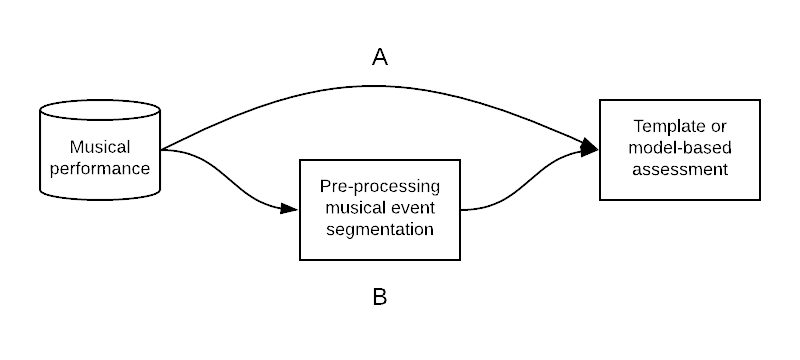
\includegraphics[width=\textwidth]{figs/blockDiags_rong/ch2_assessment.png}
\caption{The general flowchart of automatic assessment of musical performance. A: assessment for the entire music piece. B: assessment for musical event units.}
\label{fig:ch2_assessment}
\end{figure}

The automatic assessment methods can be either template-based \shortcite{Caoa, Tsai2012a, Molinaa, Bozkurta, Guptab} or model-based \shortcite{Nakanoa, Schramm2015b, Robinea, Hana, Luoa, Guptac}. The former case means that the reference performance are provided for a comparision with the target assessing performance. While the latter case indicates that the reference performance are not given, and the target performance are assessment using a pre-trained model. Regarding the templated-based assessment, the similarity calculation between the reference and target musical performance segments is usually involved. Thus we review the neural acoustic embedding technique which can faciliate the similarity calculation. A general flowchart of automatic assessment of musical performance is illustrated in \figref{fig:ch2_assessment}.

\subsection{Automatic assessment of musical performance}

We introduce the overview of the studies on general automatic assessment of musical performance in this seciton. A significant number of authors adopt the regression or classification model to predict the human rating of the musical performance with acoustic features. In this following part of this section, we firstly present the studies of automatic singing voice assessment. Then we present those of instrumental performance assessment.

\subsubsection{Automatic assessment of singing voice}
In \tabref{tab:ch2_automatic_assessment_singing}, we list the goal and methods of each work. A model-based method is presented by \shortcite{Nakanoa} for evaluating unknown melodies. The SVM is trained with semitone stability and vibrato features to classify the good and poor singers. The evaluation dataset contains 600 songs sung by 12 singers -- 6 good and 6 poor. \shortcite{Daido2014a} identifies that three features -- A-weighted power, F0 fall-down and vibrato extent, are relevant to singing enthusiasm. Then they build a regression model to predict the human rating scores of singing enthusiam by combing these three features.

As we have mentioned above, most of the works are template-based and build regression or classification model for the prediction of human rating. \shortcite{Caoa} calculate features on four categories -- intonation, rhythm, timbre brightness and vocal clarity, then adopt SVR regression model to predict the expert rating scores of the singing quality. \shortcite{Liu2011a} propose a two-step method for solfège assessment. In the first step, they use DTW to align the reference and target performance pitch tracks. In the second step, they calculate intonation and rhythm features using the aligned musical notes. Relative pitch interval and lagged tempo reference are identified respectively as the most correlated features for intonation and rhythm rating. \shortcite{Tsai2012a} model intonation rating using DTW cost between reference and target pitch tracks, model volume rating using DTW cost between reference and target logarithmic energy curves, model rhythm rating using HMM classification score between pitch strength time sequences, and predict the overall score with linear regression model by combining these three dimension ratings. 

\shortcite{Molinaa} explore both low-level and high-level features for singing voice intonation and rhythm assessment. The reference used in their work is not symbolic midi but singing audio. Low-level features are calculated based on the DTW alignment path, and high-level features are calculated on the transcribed musical notes. They calculate the correlation coefficients between each individual feature and expert rating score, and find that low-level total intonation error and high-level pitch difference are correlated with the intonation rating and low-level RMS of the alignment path is correlated with the rhythm rating. Finally, they use quadratic polynominal regression model with all the features to predict the overall singing quality. \shortcite{Bozkurta} develop a dataset and a baseline model for the singing assessment of the conservatory entrance exam. Their dataset contains 2599 piano references and 1018 singing performance of 40 different melodies. These singing performances are labeled as pass or fail categories by 3 experts. They use DTW to align the pitch tracks between the singing performance and the piano reference. The baseline is built by using a multilayer perceptron model with 3 featuers -- pitch difference histogram, DTW alignment cost and the amount of the length change of the DTW alignment. \shortcite{Guptab} construct the singing assessment model on 6 aspects - intonation accuracy, rhythmic consistency, pronunciaiton, vibrato, volume and pitch range. To avoid the alignment error caused by the intonation mistake, they use MFCC as the representation for the DTW alignment between reference and target. They also experiment cognition modeling for obtaining the perceptual relevant features. Finally, both linear regression and multilayer perceptron models are explored to predict human ratings with various feature combinations.

In the works mentioned above, the model are built to assess the singing performance in the entire musical excerpt granularity. However, several works explore the assessment of detailed musical events, such as note, expression segment and syllable. \shortcite{Mayor2006b} proposed a probablistic and rule-based method for note alignment and expression segmentation. They use HMM framework with Viterbi algorithm for the note alignment. The cost probablity is calculated by a set of heurstic rules which are defined on timing, pitch, energy, vibrato and timbre. The similar idea is adopted for expression segmentation. They define several rules for the expressions such as attack, sustain, vibrato, release and transition. The HMM topology of the expression is constrained by the note segmentation. \shortcite{Schramm2015b} construct a Bayesian classifier to assess the performing correctness of solfège note. They first transcribe the pitch track and notes for the target singing performance, and devise a special DTW algorithm to align the reference score the transcribed notes. For each assessment dimension -- note-level pitch, onset and offset, they construct Gamma probability density functions for both correct and incorrect classes. Finally, they identify the fuzzy boundary between two classes using a Bayesian classifier. In \shortcite{Guptac}'s work, they first generalize the mispronounciation rules for the singing voice of Southeast Asian English dialects. Then they use Automatic Speech Recognition system with an adapted dictionary to detect the mispronunciation.

\begin{landscape}
\mbox{}\vfill
\begin{table}[ht!]
\ContinuedFloat
\centering
\begin{tabular}{lcc}
\toprule
Authors              & Goal                                          & Methods                                                                                           \\
\midrule
\shortcite{Mayor2006b}  & Expression categorization and alignment       & \makecell{Rule-based note and\\expression alignment\\using Viterbi algorithm}         \\\hline
\shortcite{Nakanoa}     & \makecell{Singing skill evaluation\\for unknown melodies} & \makecell{Building SVM model\\to classify good and bad performance.}      \\\hline
\shortcite{Caoa}        & Singing quality evaluation                    & \makecell{Building SVM regression model\\between features and\\human rating scores.}  \\\hline

\shortcite{Liu2011a}    & Singing evaluation                            & \makecell{Using correlation coefficient\\to select the best features.}                \\\hline
\shortcite{Tsai2012a}   & Karaoke singing evaluation                    & \makecell{Building linear regression model\\for predicting the overall score.}        \\\hline
\shortcite{Molinaa}      & Singing voice assessment              & \makecell{Building nonlinear regression model\\for predicting the human rating score.}                     \\\hline
\shortcite{Daido2014a}   & Singing enthusiasm evaluation         & \makecell{Building linear regression model\\for predicting the human rating\\of singing enthusiasm.}        \\
\bottomrule   
\end{tabular}
\caption{Summary table of the previous studies on automatic assessment of singing voice.}
\label{tab:ch2_automatic_assessment_singing}
\end{table}
\vfill
\end{landscape}

\begin{landscape}
\mbox{}\vfill
\begin{table}[ht!]
\ContinuedFloat
\centering
\begin{tabular}{lcc}
\toprule
Authors              & Goal                                          & Methods                                                                                           \\
\midrule
\shortcite{Schramm2015b} & Solfège assessment                    & \makecell{Constructing Gamma probability\\density functions,\\building Bayesian classifiers\\for each note.}    \\\hline
\shortcite{Bozkurta}     & Singing voice assessment                      & \makecell{Building a Multilayer perceptron model\\for predicting the human rating.}                         \\\hline
\shortcite{Guptab}       & Singing quality evaluation                    & \makecell{Using both linear regression\\and Multilayer perceptron\\for predicting the human rating.}        \\\hline
\shortcite{Guptac}       & Singing mispronunciation detection    & \makecell{DNN-HMM lyrics-to-audio\\forced alignment,\\using an adapted dictionary\\to detect mispronunciation.} \\
\bottomrule   
\end{tabular}
\caption{Summary table of the previous studies on automatic assessment of singing voice. (continued)}
\end{table}
\vfill
\end{landscape}

\subsubsection{Automatic assessment of intrumental music performance}

In \tabref{tab:ch2_automatic_assessment_instrumental}, we list the goal and methods of each work. We have identified that in three works, the assessment is conducted at music excerpt level. Several pitch and rhythm score-independent features and score-based features are proposed in \shortcite{Vidwans2017a}'s work. A SVR regression model is experimented with various feature combinations to predict the expert ratings of Alto Saxophone performance. \shortcite{Wua} use sparse coding to learn representations in a unsupervised way on the local histogram matrix features. The learned features are used in a SVR model to predict the expert ratings for the percussive music performance. \shortcite{Pati2018a} use fully-convolutional neural networks and covolutional recurrent neural networks to predict the expert ratings for the saxophone, clarinet and flute music performance. Pitch track and logarithmic Mel band energies are adopted as the input representations of the networks. They also discuss the learned representation for the musicality dimension using network inspection techniques. 

In other works, the asessment is done at musical note-level. \shortcite{Robinea} assess the note quality of saxophone performance. They extract pitch and amplitude related features for stable, crescendo/decrescendo and vibrato notes. Then, the feature values are mapped to the expert ratings. \shortcite{Knighta} develop models to assess the trumpet performance at note-level. They use a SVM classifier to predict the expert ratings with 56 dimensional features of which are mostly spectral features. \shortcite{Luoa} build a bag-of-features plus classifciation model to detect violin performing mistake. Their note and expression segmentation are achieved using a photo resistor and four rings of surfacemounted light-emitting diodes (SMD LEDs). \shortcite{Hana} detect three types of flute performing errors -- assembeling error, fluctuated sound and mis-fingering by using handcrafted features and Random Forest classifier.

\begin{landscape}
\mbox{}\vfill
\begin{table}[ht!]
\centering
\begin{tabular}{lcc}
\toprule
Authors              & Goal                                          & Methods                                                                                           \\
\midrule
\shortcite{Robinea}  & To assess saxophone notes                     & \makecell{Extracting metrics for straight,\\crescendo/decrescendo\\and vibrato notes}                         \\\hline
\shortcite{Knighta}  & Trumpet tone quality assessment               & \makecell{Building SVM model\\to classify trumpet tone quality on 7 scales.}                                  \\\hline
\shortcite{Hana}     & \makecell{Detecting common mistakes\\of flute players}       & \makecell{Using handcrafted features, thresholding\\and Random Forest classifier\\to detect playing mistakes.} \\\hline
\shortcite{Luoa}     & \makecell{Detection of common violin\\playing mistakes}      & \makecell{Building SVM classifiers\\for detecting four types\\of violin playing mistakes.}      \\\hline
\shortcite{Vidwans2017a}  & \makecell{Assessment of student\\music performance}          & \makecell{Building SVR regression model\\for predicting the human rating score.}    \\\hline 
\shortcite{Wua}           & \makecell{Percussive\\music performance assessment}        & \makecell{Using sparse coding to learn the feature,\\then building SVR modelfor prediction.}   \\\hline
\shortcite{Pati2018a}     & \makecell{Multi-intrumental\\student music performance}                     & \makecell{Using fully-convolutional network\\or covolutional recurrent network\\for prediction.}           \\
\bottomrule
\end{tabular}
\caption{Summary table of the previous studies on automatic assessment of instrumental musical performance.}
\label{tab:ch2_automatic_assessment_instrumental}
\end{table}
\vfill
\end{landscape}


\subsection{Musical onset detection}

Musical onset detection (MOD) is aimed to automatically detect musical onsets such as musical note, singing syllable onsets, in the musical signal. Most of the MOD methods follow this pipeline -- (1) calculating audio input representation, (2) onset detection function (ODF) computation, (3) onset selection. In \tabref{tab:ch2_musical_onset}, we list the method used in each MOD work.

Various audio input representations are used for the first step of the pipeline, such as filtered logarithmic magnitude and phase spectrum \shortcite{Bello2005b,Bocka}. The former can be subdivided by the filterbank type -- Bark scale bands \shortcite{Bock2012b}, Mel scale bands \shortcite{Eybena,Schluter2014} or constant-Q bands \shortcite{Lacoste2007b,Bock2012c}.

Depending on the techniques used, we classify ODF computation methods into three categories:

\noindent\textbf{Unsupervised methods}: Methods in this category estimate ODF in an unsupervised way. Earlier methods in this category are based on calculating temporal, spectral, phase, time-frequency or complex domain features, such as energy envelope, high-frequency content, spectral difference, phase deviation and negative log-likelihoods. Bello et al. \shortcite{Bello2005b} and Dixon \shortcite{Dixon2006} both review these methods thoroughly. The state-of-the-art methods in this category are based on spectral flux feature \shortcite{Bock2012c}. Some variants such as \textit{SuperFlux} \shortcite{Bocka}, local group delay weighting \shortcite{Bock2013} are proposed to suppress the negative effect of vibrato, primarily for pitched non-percussive instruments. The advantage of these methods is that no data is needed for training the ODF, and they are computationally efficient and can often operate in online real-time scenarios.

\noindent\textbf{Non-deep learning-based supervised methods}: Some methods in this category are probabilistic model-based, such as using Gaussian autoregressive models to detect the onset change point \shortcite{Bello2005b}. Toh et al. \shortcite{ChuanTohBingjunZhangYeWang2008} propose a method using two Gaussian Mixture Models to classify audio features of onset frames and non-onset frames. Chen \shortcite{Chen2016} detect the onset candidates from two ODFs, extracted features around these candidates, then used support vector machine technique to classify them.

\noindent\textbf{Deep learning-based supervised methods}: The state-of-the-art performance in the MIREX Audio Onset Detection is defined by deep learning-based methods. Lacoste et al. \shortcite{Lacoste2007a,Lacoste2007b} are the earliest researchers who apply feed-forward or convolutional neural networks (CNNs) to esimtate the ODF. Eyben et al. \shortcite{Eybena} propose using recurrent neural networks (RNNs) with LSTM units to predict the input frames binarily as onset or non-onset. Schlüter and Böck \shortcite{Schluter2014} use the similar idea but replace RNNs by CNNs and adopt several novel deep learning techniques, which achieve the best performance in the MIREX Audio Onset Detection task. Huh et al. \shortcite{Huh2018} estimate time-to-event (TTE) or time-since-event (TSE) distributions from Mel-spectrograms by a CNN, then use them as a onset density predictor.

The last step of the pipeline -- onset selection can be done by peak-picking \shortcite{Bock2012c} algorithm.

\begin{landscape}
\mbox{}\vfill
\begin{table}[ht!]
\centering
\begin{tabular}{lc}
\toprule
Authors                                                        & Methods                                                                                           \\
\midrule
\shortcite{Bello2005b}   	& \makecell{A tutorial paper, introducing spectral feature-based,\\probability model-based and negative likelihood onset detection methods.}         \\\hline
\shortcite{Dixon2006}      	& \makecell{Another review paper, proposing a weighted phase deviation function\\and a half-wave rectified complex difference for onset detection.}  \\\hline
\shortcite{Lacoste2007a}    & \makecell{Feed-forward neural networks for onset detection.}                \\\hline
\shortcite{Lacoste2007b}    & \makecell{Convolutional neural networks for onset detecion.}  		      \\\hline
\shortcite{ChuanTohBingjunZhangYeWang2008}   & \makecell{Using GMMs model, fusion-level and\\decision-level fusion for singing onset detection.}        \\\hline
\shortcite{Eybena}   		& \makecell{Two frame size logarithmic Mel bands input,\\Bidirectional LSTMs for binary onset classification.}         		\\\hline
\shortcite{Bock2012c}      	& \makecell{Using logarithmic Constant-Q bands as input,\\and half wave rectified spectral difference as onset detection function.}      \\
\bottomrule   
\end{tabular}
\caption{Summary table of the previous studies on musical onset detection.}
\label{tab:ch2_musical_onset}
\end{table}
\vfill
\end{landscape}

\begin{landscape}
\mbox{}\vfill
\begin{table}[ht!]
\ContinuedFloat
\centering
\begin{tabular}{lc}
\toprule
Authors                                                        & Methods                                                                                           \\
\midrule
\shortcite{Bock2012b}       & \makecell{3 channels logarithmic Bark bands input,\\using single direction RNN for online onset detection.}  							\\\hline
\shortcite{Bock2013}    	& \makecell{Using local group delay (LGD) weighting of Superflux\\to suppress the false postive onsets caused by vibrato and tremolo.}   \\\hline
\shortcite{Bocka}   		& \makecell{Introducing SuperFlux, using Maximum filter\\to suppress the vibrato ripple in the spectral flux.}        	  \\\hline
\shortcite{Schluter2014}   	& \makecell{3 channels logarithmic Mel bands input,\\using convolutional neural networks as detection funcition.}         \\\hline
\shortcite{Chen2016}      	& \makecell{Multiple onset detection functions, SVM onset classification.}      										  \\\hline
\shortcite{Huh2018}      	& \makecell{Using time-to-event (TTE) or time-since-event (TSE)\\prediction for onset detection.}      \\
\bottomrule   
\end{tabular}
\caption{Summary table of the previous studies on musical onset detection. (continued)}
\end{table}
\vfill
\end{landscape}

\subsection{Text-to-speech alignment}

Text-to-speech alignment is a process that the orthographic transcription is aligned in temporal axis with the speech audio at word, syllable or phone-level. In \tabref{tab:ch2_speech_forced}, we list the method used in each text-to-speech alignment work. Most of the non-commercial alignment tools are built on HTK \shortcite{Young2006HTK} or Kaldi \shortcite{Povey2011ASRU} frameworks, such as Montreal forced aligner \shortcite{McAuliffe2017} and Penn Forced Aligner \shortcite{PennForced}. These tools implement an intermediate step of automatic speech recognition (ASR) pipeline, train the HMM acoustic models iteratively using Baum-Welch or Viterbi algorithm and align audio features (e.g. MFCCs) to the HMM monophone or triphone model. Brognaux and Drugman \shortcite{brognaux2016hmm} explore the forced alignment in a small-dataset case using supplementary acoustic features and initializing the HMM silence model by voice activity detection (VAD) algorithm. To predict the confidence measure of the aligned word boundaries and to fine-tune their time positions, Serri\'{e}re et al. \shortcite{serriere2016weakly} explore an alignment post-processing method using a deep neural network (DNN). Usually, no manually boundary labeled dataset is needed for the HMM acoustic model training which is initialized by flat-start training method \shortcite{Young2006HTK}. \shortcite{pakoci2016phonetic} experiment to train HMM acoustic model by making use of a manually boundary labeled dataset in a small-dataset scenario.

The forced alignment is a language-dependent method, in which the acoustic models should be trained by using a corpus of certain language. Another category of text-to-speech methods is language-independent, which relies on detecting the phoneme boundary change in the temporal-spectral domain \shortcite{esposito2005text,almpanidis2009Robust}. The drawback of these methods is that the segmentation accuracies are usually poorer than the language-dependent counterparts. 

\begin{landscape}
\mbox{}\vfill
\begin{table}[ht!]
\centering
\begin{tabular}{lc}
\toprule
Authors                                                        & Methods                                                                                           \\
\midrule
\shortcite{McAuliffe2017}   		& \makecell{A text-to-speech forced alignment tool built on Kaldi.}         \\\hline
\shortcite{PennForced}      		& \makecell{Another text-to-speech alignment tool build on HTK}  \\\hline
\shortcite{brognaux2016hmm}    		& \makecell{Experimenting forced alignment\\with supplementary acoustic features.}                \\\hline
\shortcite{serriere2016weakly}    	& \makecell{Forced alignment with DNN post-processing.}  		      \\\hline
\shortcite{esposito2005text}   		& \makecell{Text independent alignment\\by detecting fast transition of phone onsets.}        \\\hline
\shortcite{almpanidis2009Robust}   	& \makecell{Detecting phone boundaries using model selection techniques.}         		\\\hline
\shortcite{pakoci2016phonetic}      & \makecell{Forced alignment making use of dataset\\which has the manually labeled phone boundaries.}      \\
\bottomrule   
\end{tabular}
\caption{Summary table of the previous studies on text-to-speech alignment.}
\label{tab:ch2_speech_forced}
\end{table}
\vfill
\end{landscape}

\subsection{Lyrics-to-audio alignment}

To goal of lyrics-to-audio alignment is similar to text-to-speech alignment -- aligning the lyrics with the singing voice audio at word, syllable or phone-level. In \tabref{tab:ch2_lyrics_audio}, we list the method used in each lyrics-to-audio alignment work. Most of these works \shortcite{mesaros2008automatic, loscos1999Low, fujihara2011lyricsynchronizer, mauch2012integrating, iskandar2006syllabic,gong2015real, kruspe2015keyword, dzhambazov2015modeling} use the speech forced alignment method accompanied with music-related techniques. Loscos et al. \cite{loscos1999Low} use MFCCs with additional features and also explore specific HMM topologies to take into account of singing aspiration, silence and different pronunciation possibilities. To deal with mixed recordings, Fujihara et al. \shortcite{fujihara2011lyricsynchronizer} use voice/accompaniment separation to extract clean singing voice. They also adopt vocal activity detection, fricative detection techniques to recover the consonant information lost in the separation process. 

Additional musical side information extracted from the musical score is used in many works. Mauch et al. \shortcite{mauch2012integrating} use chord information such that each HMM state contains both chord and phoneme labels. Iskandar et al. \shortcite{iskandar2006syllabic} constrain the alignment by using musical note length distribution. Gong et al. \shortcite{gong2015real}, Kruspe \shortcite{kruspe2015keyword}, Dzhambazov and Serra \shortcite{dzhambazov2015modeling} all use syllable/phoneme duration extracted from the musical score as side information, and decode the alignment path by duration-explicit HMM models. Chien et al. \shortcite{Chien2016Alignment} introduce an approach based on vowel likelihood models. Chang and Lee \shortcite{Chang2017Lyrics} use canonical time warping and repetitive vowel patterns to find the alignment for vowel sequence. Some other works achieve the alignment at music structure-level \shortcite{muller2007lyrics} or line-level \shortcite{wang2004lyrically}.

\begin{landscape}
\mbox{}\vfill
\begin{table}[ht!]
\centering
\begin{tabular}{lc}
\toprule
Authors                                                        & Methods                                                                                           \\
\midrule
\shortcite{loscos1999Low}   				& \makecell{Forced alignment with addtional features and special HMM topologies.}         \\\hline
\shortcite{iskandar2006syllabic}      		& \makecell{Forced alignment using musical note length distribution.}  \\\hline
\shortcite{fujihara2011lyricsynchronizer}   & \makecell{Treating mixed recordings with voice/accompaniment separation,\\forced alignment with phone filler topologies.}                \\\hline
\shortcite{mauch2012integrating}    		& \makecell{Forced alignment using chord side information.}  		      \\\hline
\shortcite{gong2015real}   					& \makecell{Forced alignment with HSMM model using vowel duration information.}        \\\hline
\shortcite{kruspe2015keyword}   			& \makecell{Forced alignment with duration-explicit HMM model.}         		\\\hline
\shortcite{dzhambazov2015modeling}      	& \makecell{Forced alignment with duration-explicit HMM model.}      \\\hline
\shortcite{Chien2016Alignment}      		& \makecell{A method based on vowel likelihood model.}      \\\hline
\shortcite{Chang2017Lyrics}      			& \makecell{A method based on canonical time wraping and repetitive vowel patterns.}      \\\hline
\shortcite{muller2007lyrics}      			& \makecell{Structure-level DTW alignment.}      \\\hline
\shortcite{wang2004lyrically}      			& \makecell{Line-level alignment making use of rhythm, chrous and singing voice detection.}      \\
\bottomrule   
\end{tabular}
\caption{Summary table of the previous studies on lyrics-to-audio alignment.}
\label{tab:ch2_lyrics_audio}
\end{table}
\vfill
\end{landscape}

\subsection{Neural acoustic embeddings}

Neural acoustic embeddings is a technique to convert variable-length acoustic sequence into fixed-length vector using neural networks. It is a common technique that is adopted in speech field, and applied to various tasks such as Query-by-Sample search and speech recognition. In those tasks that involve measuring the similarity between speech segments, acoustic embeddings generated from neural networks allows a more efficient and accurate computation because the alignment between variable-length speech segments can be avoided. In \tabref{tab:ch2_neural_acoustic}, we list the method used in each speech neural acoustic embedding work.

To embed variable-length representation of acoustic word segment such as MFCCs into fixed-length vector. \shortcite{Kampera} experiment two neural network architectures -- classification CNN and Siamese CNN. Softmax units are used in the output layer of the classification CNN, which allows it to classify input word segment into word categories in a fully-suprvised fashion. The vector output from the last CNN layer is taken as the word embedding. The hinge cosine triplet loss is used by the Siamese CNN of which the network training is done in a semi-supervised way. The penultimate layer of the Siamese CNN is taken as the word embedding such that the dimension is adjustable. RNN is a natural choice for the sequential data modelling. In the work of Settle et al. \shortcite{Settle2016a}, the CNN is replaced by RNN in both classification and Siamese architectures. A weighted random sampling method is also devised to accelerate the Siamese RNN training. The acoustic word embeddings learned from the Siamese RNN is then used in a Query-by-Example search task with a small training dataset \shortcite{Settlea}.

Apart from exploring different neural network architectures to obtain an efficient word embedding, we can also take advantage of multiple information sources. Zeghidour et al. \shortcite{Zeghidour2016a} jointly learn phoneme and speaker embeddings by a single Siamese network which minimize simutanously two objectives. In the work of He et al. \shortcite{Hea}, acoustic word segment and text word segment are embeded by two different RNNs. The embeddings of the two different sources are projected into a common space and used in the objective function in a mixed way. 

Neural acoustic embeddings can also be learned in an unsupervised way. Chung et al. \shortcite{Chungb} adopt sequence-to-sequence model commonly used in natural language processing tasks to learn the word embeddings. They experiment skipgrams and continous bag-of-words training methods and show a superior performance than simply reconstructing the input representation \shortcite{Chungc} 

\begin{landscape}
\mbox{}\vfill
\begin{table}[ht!]
\centering
\begin{tabular}{lc}
\toprule
Authors                                                        & Methods  \\
\midrule
\shortcite{Kampera}   		& \makecell{Generating acoustic word embeddings using CNN and Siamese network.}    \\\hline
\shortcite{Settle2016a}     & \makecell{Similar to \shortcite{Kampera}, but using RNN rather than CNN.}  \\\hline
\shortcite{Settlea}   		& \makecell{Using Siamese network word embeddings\\for Query-by-Example search task.}     \\\hline
\shortcite{Zeghidour2016a}  & \makecell{Using Siamese network to jointly\\learn phoneme and speaker embeddings.}   \\\hline
\shortcite{Hea}   			& \makecell{Embedding acoustic words and character sequences\\simutanously by multi-objectives.}      \\\hline
\shortcite{Chungb}    		& \makecell{Learning acoustic word embeddings\\in an unsupervised way using sequence-to-sequence model.}  		      \\\hline
\shortcite{Chungc}      	& \makecell{Similar to \shortcite{Chungb}, but using skipgrams\\and continuous bag-of-words trainings rather than reconstruct the input.}      \\
\bottomrule   
\end{tabular}
\caption{Summary table of the previous studies on neural acoustic embeddings.}
\label{tab:ch2_neural_acoustic}
\end{table}
\vfill
\end{landscape}

\subsection{Evaluation metrics}

A simple evaluation metric for onset detection is adopted in many state of the art works \shortcite{Eybena,Bock2012c,Bock2012b,Bock2013,Bocka,Schluter2014}. We use the same metric for our evaluation. To define a correctly detected onset, a tolerance threshold of $\tau=25$ms is chosen. If the detected onset $o_d$ lies within the tolerance of its ground truth counterpart $o_g$: $|o_d-o_g|<\tau$, we consider that it's correctly detected. A more strict metric can be defined by requiring that the label of the detected onset and that of the ground truth are identical. The F-measure is a number between 0 and 1 calculated as the harmonic mean of the precision and recall. Precision is the ratio between the number of correctly detected onsets and all detected onsets, and recall is the ratio between the number of correctly detected onsets and the total annotated onsets.  

\begin{equation}
\textrm{Precision} = \frac{\textrm{number of correctly detected onsets}}{\textrm{number of all detected onsets}}
\end{equation}

\begin{equation}
\textrm{Recall} = \frac{\textrm{number of correctly detected onsets}}{\textrm{number of total annotated onsets}}
\end{equation}

\begin{equation}
\textrm{F-measure} = 2 \cdot \frac{\textrm{Precison} \cdot \textrm{Recall}}{\textrm{Precision} + \textrm{Recall}}
\end{equation}

The metric presented above can also be used to evaluate alignment algorithm. However, we apply another metric for the alignment evaluation -- percentage of correct segments, which is defined as the ratio between the duration of correctly aligned segments and the total duration of the music piece. This metric has been suggested by Fujihara et al. \shortcite{fujihara2011lyricsynchronizer} in their lyrics alignment work.

\begin{equation}
\begin{split}
\textrm{Percentage of correct segments} =\\\frac{\textrm{duration of correctly aligned segments}}{\textrm{total duration of the music piece}}
\end{split}
\end{equation}

In this dissertation, the acoustic embedding will be always used as a representation for the similairy (distance) computation. Thus the evaluation of acoustic embedding needs to be done with the help of a simlarity (distance) measure. The ground truth label is set to 1 if two singing segments belong to the same class (phoneme, special pronunciation, etc.), 0 vice versa. We report the average precision (AP) between the pairwise similarities of the segments and the ground truth as the evaluation metric. The AP is used previously to evaluate speech word acoustic embedding \cite{Kampera,Settle2016a}. It is also suggested as the metric for imbalanced test set \cite{Davis2006}, which is the case of the pronunciation aspect evaluation.

AP is defined as the area under the precision-recall curve. In pratice, it is calculated by a finite sum \shortcite{Su2015}:
\begin{equation}
\textrm{Average precision} = \sum_{i=1}^{n} p(i)\Delta r(i)
\end{equation} 
where $p(i)$ is the precision in index $i$, and  $\Delta r(i)$ is the change in recall from $i-1$ to $i$.

In \figref{fig:ch2_average_precision}, we illustrate an example of calculating AP for the pairwise similarities of three segments, e.g. segment 1 and 2 belong to the class A, and their ground truth similarity and calculated similarity are respectively 1.0, 0.8.

\begin{figure}[ht!]

\includegraphics[width=\textwidth]{figs/blockDiags_rong/ch2_average_precision.png}
\caption{An example of calculating average precision for the pairwise similarities of three segments.}
\label{fig:ch2_average_precision}
\end{figure}